\begin{frame}{Object Storage - What is it}
\begin{columns}
    \begin{column}{0.47\textwidth}
    \begin{block}{Object Storage}
        \begin{itemize}
            \item Stores data in  flat structure
            \item High Performance with unstructured data
            \item Flexible data sizes, very small/very large
            \item RESTful API
        \end{itemize}
    \end{block}
    \end{column}
    \begin{column}{0.47\textwidth}
    \begin{figure}
        \centering
        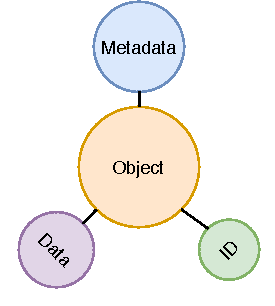
\includegraphics{img/object.pdf}
        \caption{Object Structure}
        \label{fig:my_label}
    \end{figure}
    \end{column}
\end{columns}
\end{frame}
\note{So this is a way to deal with unstructured data, in a sensible way that makes sense. Store the data as an object with a rich metadata that describes information about it, and associate an ID to it.}
\begin{frame}{Object Storage - Image Example}
    \begin{columns}
    \begin{column}{0.47\textwidth}
    \begin{figure}
        \centering
        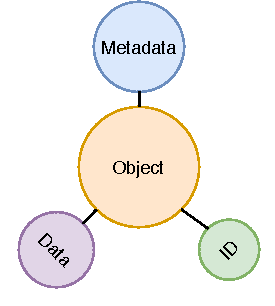
\includegraphics{img/object.pdf}
        \caption{Object}
        \label{fig:my_label}
    \end{figure}
    \end{column}
    \begin{column}{0.47\textwidth}
    \begin{figure}
        \centering
        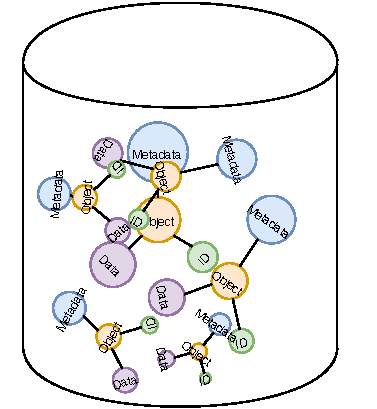
\includegraphics[width=\textwidth,height=0.55\textheight,keepaspectratio]{img/pool.pdf}
        \caption{Image Pool}
        \label{fig:my_label}
    \end{figure}
    \end{column}
\end{columns}
\end{frame}
\note{Instead, we can have a Pool called images and place the images inside that pool as objects, with metadata attached identifying what the image is instead.  Now we can just put images in the pool without having to worry where to put them. And when we want to get the image with a Dog at the Beach, we can look through the metadata and find images with that included that information. }

\begin{frame}{Object Storage - Pros and Cons}
\begin{columns}[t]
    \begin{column}{0.47\textwidth}
    \begin{block}{Pros}
        \begin{itemize}
            \item Flat structure
            \item Ideal for unstructured data
            \item Cloud Native (RESTful API)
            \item Scales 
            \item Chunking
        \end{itemize}
    \end{block}
    \end{column}
    \begin{column}{0.47\textwidth}
    \begin{block}{Cons}
        \begin{itemize}
            \item Not as good with structured data
            \item Harder to browse and interact
            \item Editing Objects
        \end{itemize}
    \end{block}
    \end{column}
\end{columns}
\end{frame}
\note{So the flat structure makes the retrieval of data a lot easier and efficient, due to the way you access the data it is perfect for cloud integration. It scales easily with limited overhead, no servers dedicated to file structure. There are cons of course it is not a magic bullet to storage issues, most obvious is structure data, the fact it is not as easy to browse an object store and interact with it there are applications that help this problem however, DosNa being one, and you can't append to an object you need to read and write the whole thing.}
